% This LaTeX file contains your written lab questions.  You may answer these
% questions just by inserting your answer into this document.  You are not
% *required* to do your homework in LaTeX, but it's quite likely to be easier
% than e.g. the equation editor in OpenOffice Writer or Microsoft Word.
\documentclass{article}

\usepackage{amsmath}
\usepackage{amssymb}
\usepackage{algpseudocode}
\usepackage{algorithmicx}
\usepackage{tikz}

\usetikzlibrary{positioning}

\begin{document}

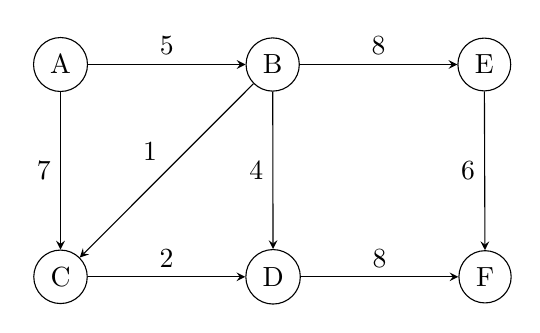
\begin{tikzpicture}[node distance=20mm and 20mm]
    \tikzstyle{vertex}=[circle,draw]
    \tikzstyle{edge}=[-stealth]

    \node[vertex] (A) {A};
    \node[vertex] (B) [right=of A] {B};
    \node[vertex] (C) [below=of A] {C};
    \node[vertex] (D) [right=of C] {D};
    \node[vertex] (E) [right=of B] {E};
    \node[vertex] (F) [right=of D] {F};

    \draw[edge] (A) to node[above] {5} (B);
    \draw[edge] (A) to node[left] {7} (C);
    \draw[edge] (B) to node[above left] {1} (C);
    \draw[edge] (B) to node[left] {4} (D);
    \draw[edge] (B) to node[above] {8} (E);
    \draw[edge] (C) to node[above] {2} (D);
    \draw[edge] (D) to node[above] {8} (F);
    \draw[edge] (E) to node[left] {6} (F);
\end{tikzpicture}

\vspace*{5mm}\par\textbf{Problem 1.} Perform a breadth-first search of the graph starting from vertex A.  Give the number of steps to reach \emph{every} other vertex.  Additionally, give the order in which the vertices are \emph{first} witnessed; that is, give the order in which they first enter the queue (and not necessarily the order in which they are explored).\par

%%%%%%%%%%%%%%%%%%%%%%%%%%%%%%%%
%% TODO: put your answer here %%
%%%%%%%%%%%%%%%%%%%%%%%%%%%%%%%%

1 step: Vertex A, Vertex C

2 steps: Vertex D, Vertex E

3 steps: Vertex F

A enters the Queue; B and C then enter the Queue as they are neighbors of A;
D is neighbor of both B and C and E is the neighbor of B so they both
enter the Queue; Lastly, F is neighbors with both D and E so it enters the
Queue next.

\vspace*{10mm}\par\textbf{Problem 2.} Use Dijkstra's algorithm on this graph starting from vertex A.  Give the cost of the least-cost path to \emph{every} other vertex.  Additionally, give the order in which the vertices are \emph{first} witnessed; that is, give the order in which they first enter the queue (and not necessarily the order in which they are explored).\par

%%%%%%%%%%%%%%%%%%%%%%%%%%%%%%%%
%% TODO: put your answer here %%
%%%%%%%%%%%%%%%%%%%%%%%%%%%%%%%%
A-B: Weight 5

A-C: Weight 6

A-D: Weight 8

A-E: Weight 13

A-F: Weight 16

A starts in the priority Queue; B and C enter the priority Queue with weight
paths of 5 and 7; Then C (from B), D (from B), D (from C), and E are entered
into the Queue with weights 1, 4, 2, 8. There is a new lowest weight path from
A to C of 6, and the path from B to C to D is less weight that from B to D, so the
A to D lowest weight path is 8. The lowest weight path from A to E is through B
with a weight of 13; Lastly, F is entered into the Queue and has a lowest weight
path from A to B to C to D to F of 16.
\vspace*{10mm}\par\textbf{Problem 3.} Give two valid topological sorts of this graph.\par

%%%%%%%%%%%%%%%%%%%%%%%%%%%%%%%%
%% TODO: put your answer here %%
%%%%%%%%%%%%%%%%%%%%%%%%%%%%%%%%
A, B, C, D, E, F

A, B, C, E, D, F

\end{document}
